\documentclass[11pt,a4paper]{article}
\usepackage[T1]{fontenc}
\usepackage[utf8]{inputenc}
\usepackage{lmodern,microtype,amsmath,amssymb,booktabs,longtable,array,graphicx,textcomp}
\newcommand{\euro}{\texteuro}
\usepackage[margin=22mm]{geometry}
\usepackage{xcolor,fancyhdr,enumitem,tikz}
\usetikzlibrary{arrows.meta,positioning}
\definecolor{navy}{HTML}{0F1E2E}
\definecolor{teal}{HTML}{0D8080}
\definecolor{ice}{HTML}{EEF5F5}
\definecolor{gold}{HTML}{B8860B}
\usepackage[colorlinks=true,linkcolor=teal,urlcolor=teal,citecolor=teal]{hyperref}
\hypersetup{pdftitle={Mini-IPHOREOS Extended System: Tutorial},pdfauthor={Mini-IPHOREOS project}}
\pagestyle{fancy}\fancyhf{}\fancyhead[L]{\small\textcolor{teal}{MINI-IPHOREOS EXTENDED SYSTEM / TUTORIAL}}
\fancyfoot[L]{\small Cognitive architecture, desktop simulation}\fancyfoot[R]{\thepage}
\setlength{\headheight}{15pt}
\setlength{\parindent}{0pt}\setlength{\parskip}{6pt}
\setlist{itemsep=3pt,topsep=4pt}
\newcommand{\code}[1]{\texttt{\detokenize{#1}}}
\newcommand{\notice}[1]{\par\noindent\colorbox{ice}{\parbox{.95\linewidth}{\vspace{2pt}#1\vspace{2pt}}}\par\vspace{4pt}}
\setlength{\emergencystretch}{2em}
\begin{document}

\begin{titlepage}
\textcolor{teal}{\large IPHOREOS / CONCEPT--EVENT--CONTEXT--POLICY}\par
\vspace{14mm}
{\Huge\bfseries\color{navy} Mini-IPHOREOS\\[3mm] Extended System -- Illustrated tutorial\par}
\vspace{5mm}
{\Large A minimal cognitive architecture for estimating, interpreting and acting in a wall-approach experiment\par}
\vspace{7mm}
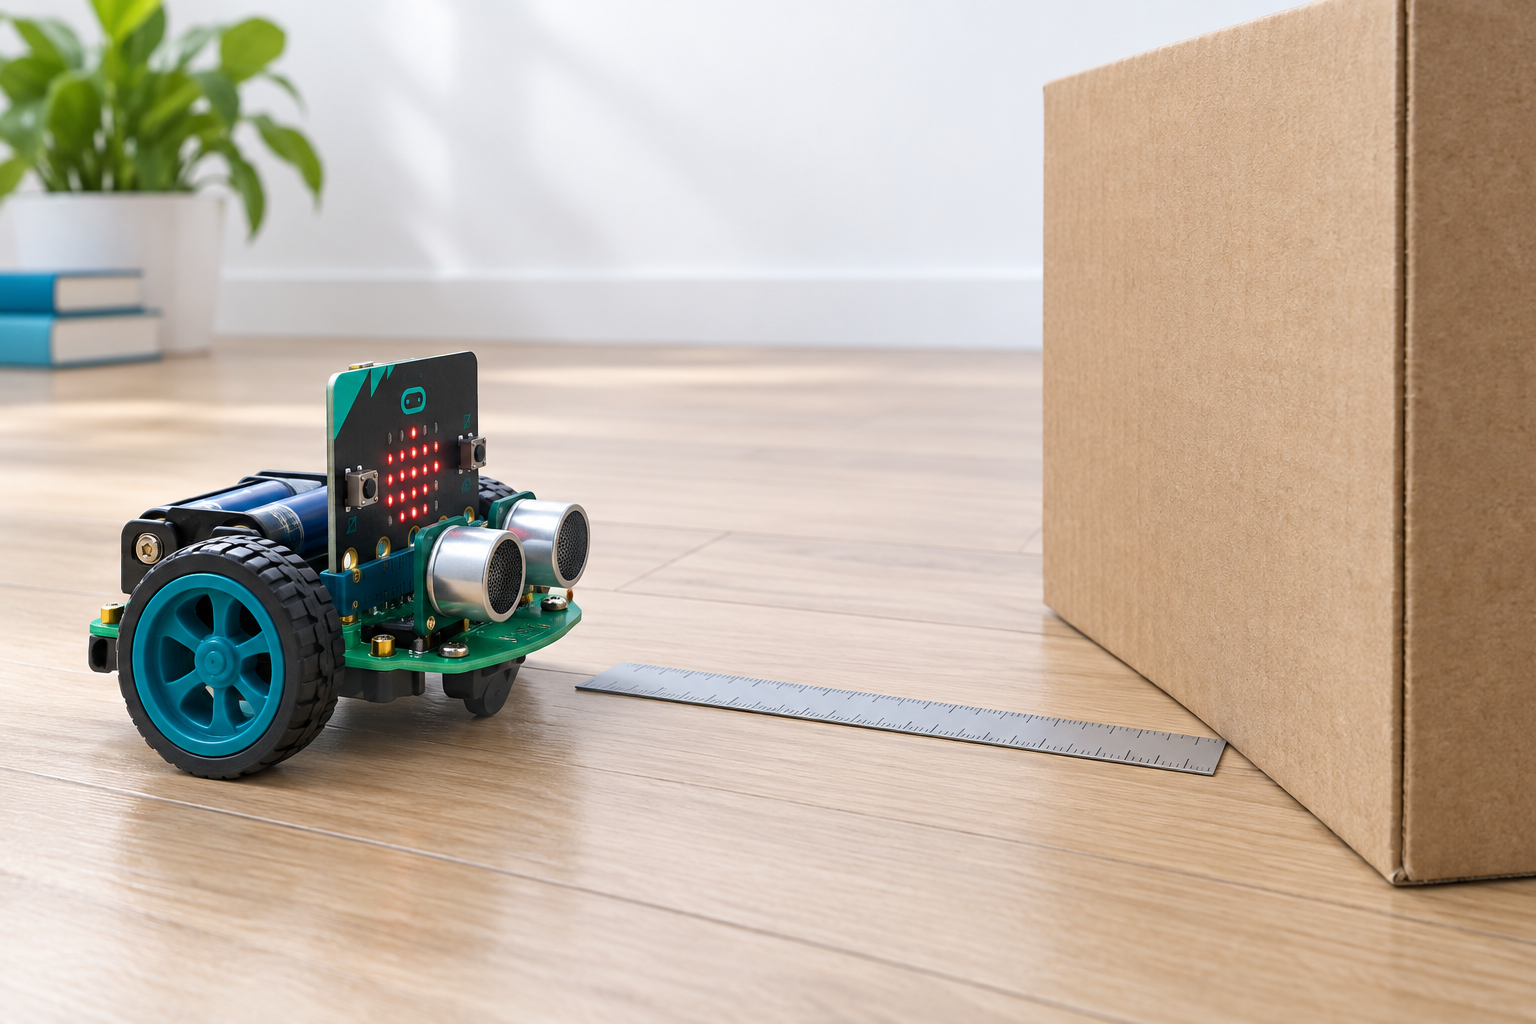
\includegraphics[width=\linewidth,height=70mm,keepaspectratio]{baseline_v1/assets/robot_concept.png}
\par{\small AI-generated concept illustration, shared with the Baseline system; not a photograph or an assembly drawing.\par}
\vspace{7mm}
\colorbox{ice}{\parbox{.95\linewidth}{\textbf{EXTENDED SYSTEM VERSION} -- a desktop Python prototype evaluated in simulation. Neither physical deployment nor autonomous discovery of new concepts is claimed.}}\par
\vspace{5mm}
This tutorial walks through what the Extended system (called \code{EXT1} in the code and file names) adds over the Baseline system (\code{V1}), how to run it, what the results show across all four development milestones -- fair baselines and a short-horizon planner; context memory and change detection; an explicit sensor-bias reference; and a frozen held-out evaluation -- concretely what moving from this simulation to a physical trial would involve, and, as a later, separate pass, the \emph{Transfer system}: a cross-task test of Objective~O3 (Section~\ref{sec:tut-transfer}).

\textbf{Companion materials:} full equation derivations are in \href{Mathematical_Model_EXT1.pdf}{Mathematical\_Model\_EXT1.pdf}. Three silent, captioned video walkthroughs are in \code{Mini_IPHOREOS_EXT1_Video/}.

\vfill
Prepared for Florent Ouabo Kamkumo\\
3 October 2026 / Extended System Milestone 4 tutorial, LaTeX edition\\
\textbf{Note on format:} this release's tutorial is produced as a \LaTeX\ document rather than the earlier HTML/PDF pipeline (\code{Tutorial_EXT1_EN.html}, now superseded and no longer updated). All content is reproduced here, plus material the HTML version never had (Sections~8--11).
\end{titlepage}
\tableofcontents
\newpage

\section{The Extended system: what changes}
Mini-IPHOREOS's Baseline system estimates distance and applies fixed rules. The Extended system jointly estimates distance and effective speed, maintains probabilities over two movement contexts, and selects an action using an objective that combines progress, cost and information.

\begin{center}\small
\begin{tabular}{p{.45\linewidth}p{.45\linewidth}}\toprule
Preserved from the Baseline system & What the Extended system changes\\\midrule
Scalar distance estimate & Distance, speed and joint uncertainty\\
Normal/careful: manual setting & Normal/slow: inferred environmental hypotheses\\
Movement rules & Comparison of candidate actions\\
Current state & Belief and event log\\
\bottomrule
\end{tabular}\end{center}

The target distance is 25~cm, with an acceptable band of 21--29~cm. Ground truth belongs to the simulator; the controller receives only noisy measurements, time and calibration parameters.

\textbf{Keeping the versions separate.} \code{baseline_v1/} contains the reference copy of the Baseline system; its files were checked against SHA-256 hashes and are never modified by Extended-system development. The extension lives in \code{cognitive/}, \code{experiments/} and \code{results_ext1/}.

\textbf{The whole system, in one loop.} Every section from here on explains one box or one arrow below -- worth seeing the whole shape once before the detail:
\begin{center}
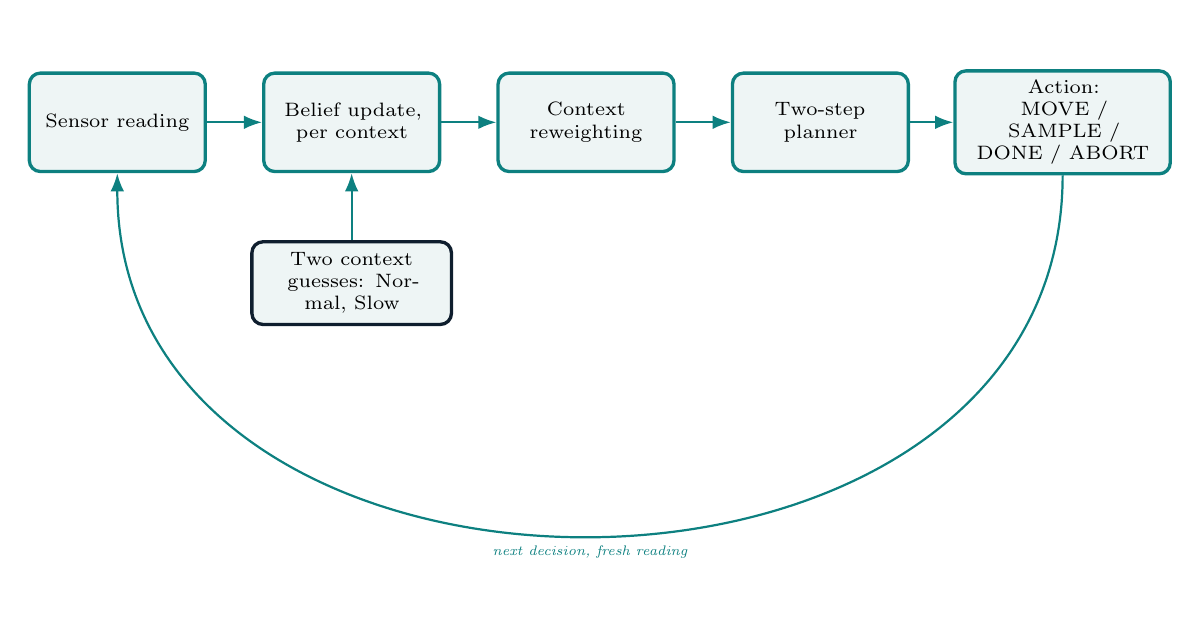
\begin{tikzpicture}[
  box/.style={rectangle,rounded corners,draw=teal,very thick,fill=ice,text width=2.0cm,align=center,minimum height=1.25cm,font=\scriptsize},
  hyp/.style={rectangle,rounded corners,draw=navy,very thick,fill=ice,text width=2.3cm,align=center,minimum height=1.05cm,font=\scriptsize},
  arr/.style={-{Latex[length=2.3mm]},thick,teal}
]
\node[box] (sensor) {Sensor reading};
\node[box,right=0.7cm of sensor] (update) {Belief update, per context};
\node[box,right=0.7cm of update] (reweight) {Context reweighting};
\node[box,right=0.7cm of reweight] (plan) {Two-step planner};
\node[box,right=0.55cm of plan,text width=2.5cm] (action) {Action:\\MOVE / SAMPLE /\\DONE / ABORT};
\node[hyp,below=0.85cm of update] (hyp) {Two context guesses: Normal, Slow};
\draw[arr] (sensor) -- (update);
\draw[arr] (update) -- (reweight);
\draw[arr] (reweight) -- (plan);
\draw[arr] (plan) -- (action);
\draw[arr] (hyp) -- (update);
\draw[arr] (action.south) to[out=-90,in=-90,looseness=1.3] node[below,font=\tiny\itshape]{next decision, fresh reading} (sensor.south);
\end{tikzpicture}
\end{center}
\textit{\small One decision = one pass around this loop: Sections~\ref{sec:tut-model} (belief and context), \ref{sec:tut-decisions} (the planner and the action).}

\section{Concepts, events and contexts}
\textbf{The loop:} observation $\to$ distance/speed belief $\to$ predictive relations $\to$ selected option $\to$ next observation $\to$ realised event.

\textbf{Operational concepts.} The log explicitly records two relations: "the target is compatible with my belief" and "this pulse should produce this displacement." Their forms are defined by the designer; calibration estimates speeds and the online loop updates beliefs. The system does not discover a conceptual vocabulary.

\textbf{Intended option and realised event.} \code{intended_option} is MOVE, SAMPLE, DONE or ABORT. \code{realised_event} describes an initial reading, an observation after movement, a stationary reading, an unexpected outcome, an unusable reading or target verification.

\textbf{Inferred context.} The normal and slow families are predefined, with calibrated speeds near 8 and 3~cm/s. The filter updates their probabilities without ever receiving the simulator's true context; no selected family is certain, evidence of a change must accumulate in the observations. The Baseline system's careful setting is a control preference, not a hypothesis about the floor -- the Extended system distinguishes these meanings.

\textbf{Memory (in the ordinary sense).} The event log connects observations, beliefs, options and outcomes and supports analysis. This is distinct from, and predates, the persistent per-context \emph{library} introduced in Section~\ref{sec:tut-memory}.

\section{Model and estimation}
\label{sec:tut-model}
The state is $x=(d,v)$, distance and speed. The discrete context is normal or slow; a Gaussian distribution is maintained for each context and combined using probability weights. In picture form, two running speed guesses held at once, each a bump of uncertainty, weighted by how likely that context currently seems (starting split 0.8/0.2):
\begin{center}
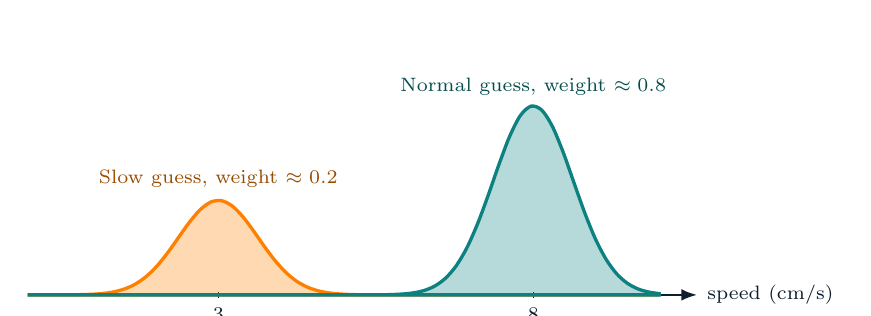
\begin{tikzpicture}[scale=0.8]
\draw[-{Latex[length=2mm]},thick,navy] (0,0) -- (10.6,0) node[right,font=\scriptsize]{speed (cm/s)};
\draw[navy] (3,0.05) -- (3,-0.05) node[below,font=\scriptsize]{3};
\draw[navy] (8,0.05) -- (8,-0.05) node[below,font=\scriptsize]{8};
\draw[orange,very thick,fill=orange,fill opacity=0.3,domain=0:10,samples=60,smooth]
  plot ({\x},{1.5*exp(-((\x-3)*(\x-3))/0.8)}) -- (10,0) -- (0,0) -- cycle;
\draw[teal,very thick,fill=teal,fill opacity=0.3,domain=0:10,samples=60,smooth]
  plot ({\x},{3.0*exp(-((\x-8)*(\x-8))/0.8)}) -- (10,0) -- (0,0) -- cycle;
\node[orange!60!black,font=\scriptsize] at (3,1.85) {Slow guess, weight $\approx0.2$};
\node[teal!60!black,font=\scriptsize] at (8,3.3) {Normal guess, weight $\approx0.8$};
\end{tikzpicture}
\end{center}
\textit{\small Sketch, not to calibrated scale. As readings arrive, whichever guess predicts them better wins weight -- the mixture narrows toward one spike.}
\begin{center}\colorbox{ice}{\parbox{.9\linewidth}{\centering
$d'=d-v\Delta t-c+\text{noise}$\\[2pt]
$v'=\rho v+(1-\rho)m_{\text{context}}+\text{noise}$\\[2pt]
$y=d+b+\text{measurement noise}$}}\end{center}
Here $c$ is mean coasting distance and $b$ is calibrated sensor bias; $\rho=0.80$. At each movement, a transition matrix with diagonal entries 0.96 allows context changes. Updates combine moment mixing, linear prediction and Kalman correction; normalised likelihoods update context weights. Repeated stationary readings do not artificially trigger context transitions (Belief tests check this directly).

Synthetic calibration is separate: seed 1701, 160 readings at four distances, and 80 pulses per speed family. Labels are available during supervised calibration but never supplied to the controller during evaluation.

\notice{\textbf{Identifiability.} With a single sensor $y=d+b+\nu$, unknown absolute distance and unknown constant bias remain confounded -- no amount of filtering resolves this on its own. Section~\ref{sec:tut-bias} adds the explicit reference that does.}

\section{Decisions and control limits}
\label{sec:tut-decisions}
After each valid reading, the candidate pulse durations are 0~s (stay and measure), 0.12~s and 0.24~s. A duration is excluded if its predicted lower distance bound, including uncertainty and a 0.5~cm margin, falls below 21~cm.

\textbf{A two-step planner, not a one-step one.} The controller enumerates \emph{pairs} of durations $(dt_1,dt_2)$ -- nine combinations -- rolls the belief forward through both steps without touching the real belief, and scores the pair as a whole. Only the first duration of the best-scoring pair is executed; the controller re-plans from the next real observation.
\begin{center}\small\colorbox{ice}{\parbox{.92\linewidth}{
Score$(dt_1,dt_2)$ = [(predicted distance after both steps $-$ 25)$^2$ + predicted variance] / 400\\
\hspace*{2em}+ 0.08 $\times$ (cost of $dt_1$) + 0.08 $\times$ (cost of $dt_2$) $-$ 0.8 $\times$ expected information from $dt_1$\\
\hspace*{2em}+ 1.0, added only to the "measure, measure" pair, and only when some safe pair would have moved the robot more than 1~cm}}\end{center}
That last term is the explicit no-progress cost: a pure "measure twice" plan is no longer allowed to look optimal purely because moving briefly raises predicted variance, whenever a safe alternative would actually make progress. A one-step planner could previously keep choosing to wait indefinitely, particularly with information-seeking off; this is a heuristic fix for an identified failure, not a proof that stalling is impossible in every situation.

Three consecutive readings satisfying $|\hat d-25|+1.64\sigma\leq4$ lead to DONE (correlated, not three independent validations). Three consecutive invalid/inconsistent readings lead to ABORT. Limits: 80~s, 100 movements, 350 decisions.

\textbf{A fair rule-based comparator.} The Baseline system's original controller only ever offers a fixed 0.12~s pulse, so it could never show what a wider action menu is worth on its own. \code{v1_fair} keeps the Baseline system's rule-based philosophy -- the same verification thresholds, the same invalid-reading and progress-abort handling, no joint speed estimation -- but chooses from the same three-value duration menu, taking the longest duration that still clears the overshoot safety margin. The Baseline system's single-pulse rule is the special case of this rule when only 0.12~s is offered. Full derivations, with a worked numerical example, are in \href{Mathematical_Model_EXT1.pdf}{the math companion}, Sections~7--9.

\section{Run and explore the project}
Open PowerShell in \code{Mini_IPHOREOS_EXT1}. For a fresh installation:
\begin{verbatim}
python -m pip install -r requirements.txt
python -B -m pytest -q -p no:cacheprovider tests
python -B experiments/run_simulation.py --trials 100
\end{verbatim}
This writes episodes to \code{results_ext1/}: six fairness-comparison scenarios (\code{normal}, \code{slow}, \code{switch}, \code{recovery}, \code{dropout}, \code{bias}) plus diagnostic-only scenarios (\code{repeated}, \code{intermediate}, \code{bias_random}, \code{outlier} -- Sections~\ref{sec:tut-memory}, \ref{sec:tut-bias}, \ref{sec:tut-heldout}), nine policies, 100 seeds per combination.

For a genuinely held-out evaluation on seeds never used during development (Section~\ref{sec:tut-heldout}):
\begin{verbatim}
python -B experiments/run_simulation.py --trials 100 \
    --seed-start 50000 --out-dir results_ext1_heldout
python experiments/compare_heldout.py
\end{verbatim}

\begin{center}\small
\begin{tabular}{p{.32\linewidth}p{.6\linewidth}}\toprule
File & Purpose\\\midrule
\code{calibration*.csv/json} & Synthetic calibration data and estimated parameters\\
\code{trials.csv} & One row per episode, including failures\\
\code{summary.csv} & Aggregated results, six fairness scenarios\\
\code{reconvergence*.csv} & Per-segment speed-reconvergence timing (\code{repeated})\\
\code{bias_reference_summary.csv} & Bias-reference cost/accuracy/recovery (\code{bias}, \code{bias_random})\\
\code{outlier_summary.csv} & Robustness under corrupted readings (\code{outlier})\\
\code{trace_*.json} & Event log and simulator truth for seed 10000 (or 50000 for held-out)\\
\code{manifest.json} & Seeds, limitations and source hashes\\
\bottomrule
\end{tabular}\end{center}
When reading a trace, distinguish \code{simulator_*} fields (truth, never available to the controller) from the controller's own output.

\section{Results and interpretation}
\label{sec:tut-results}
Success means DONE with true distance between 21 and 29~cm.
\begin{center}\scriptsize
\begin{tabular}{lrrrrrrrr}\toprule
Scenario & Baseline & Baseline fair & Adaptive & Ad.\ no-info & Extended no-info & Extended & +memory & +fast\\\midrule
normal & 100\% & 100\% & 100\% & 100\% & 100\% & 100\% & 100\% & 100\%\\
slow & 40\% & 10\% & 100\% & 0\% & 0\% & 100\% & 100\% & 100\%\\
switch & 50\% & 16\% & 97\% & 7\% & 8\% & 97\% & 97\% & 97\%\\
recovery & 100\% & 99\% & 99\% & 98\% & 99\% & 100\% & 100\% & 100\%\\
dropout & 94\% & 97\% & 97\% & 95\% & 94\% & 97\% & 97\% & 97\%\\
bias & 99\% & 92\% & 83\% & 98\% & 98\% & 86\% & 86\% & 86\%\\
\bottomrule
\end{tabular}\end{center}

\textbf{Fair-baseline check.} \code{v1_fair} completes the normal scenario in about half as many moves as the original Baseline system, confirming the Baseline system's extra moves were partly an artefact of its narrower action set. But a wider menu is not free: in \code{slow}/\code{switch}, \code{v1_fair} does noticeably \emph{worse} than the Baseline system (10\%/16\% vs.\ 40\%/50\%) -- committing to the longer 0.24~s pulse on the Baseline system's fixed, uncalibrated-for-this-regime speed overshoots by more than the short pulse would have. A wider action menu only pays off when paired with a dynamics estimate that can tell it is safe to use.

\textbf{Context versus plain adaptation.} The adaptive filter without discrete contexts, using the same information term, achieves 100\%/97\% on \code{slow}/\code{switch} -- similar to the Extended system. These single-switch scenarios do not establish a distinct advantage of the contextual layer; Section~\ref{sec:tut-memory} reports the experiment that actually isolates that question.

\textbf{The bias pattern that motivated Section~\ref{sec:tut-bias}.} Under unknown bias, the information-seeking policies did markedly worse than their no-information counterparts (the Extended system 86\% vs.\ 98\% for \code{ext1_no_information}) -- flagged in Milestone~1 as unresolved. Section~\ref{sec:tut-bias} explains why and fixes it.

\section{Context memory: a negative result, a diagnosis, and a fix}
\label{sec:tut-memory}
This section is the most scientifically interesting part of the Extended-system line of work: a clean hypothesis, a genuine failure to confirm it, a diagnosis found by tracing individual decisions rather than guessing, and a targeted fix that then worked.

\textbf{The hypothesis.} Once a regime has been experienced, recognising it again later should let the controller adapt faster than estimating its dynamics from scratch a second time -- faster \emph{reuse}, not merely accurate classification. Testing this needed the \code{repeated} scenario: normal/slow alternating every 8 moves within one long episode.

\textbf{Attempt 1: a persistent library (negative result).} Each context's mean-reversion target was a \emph{fixed} calibration constant, continuously blended across contexts by the mixing step -- nothing about a context's speed persisted once belief shifted away from it. \code{ext1_memory} adds a separate, persistent per-context record, updated only when confidently active, used as the mean-reversion target instead. Measured on \code{repeated}, this did not help -- if anything, reconvergence was slightly slower and less reliable. A follow-up fix for a hypothesised cause (the library's own uncertainty shrinking until uncorrectable) made no measurable difference across a five-point parameter sweep.

\textbf{The diagnosis.} Tracing individual decisions showed why: reconvergence time is dominated by how long the \emph{context weight} takes to swing back above the confidence gate after a switch -- governed by the fixed transition matrix and the per-reading likelihood -- not by how accurate the speed estimate is once that weight has arrived. The library only ever changed the latter. The bottleneck was recognition speed, not estimation precision.

\textbf{Attempt 2: recognise, then reuse directly.} \code{ext1_memory_fast} adds a change-point detector accumulating evidence that a challenger context fits recent readings better, using the \emph{pure} observation likelihood (no prior weighting) so a single noisy reading cannot trigger anything -- only a sustained run of evidence can. Once the accumulated evidence crosses a threshold, and only if that context's library is mature, the controller performs a discrete reset: jump the context weight up and seed the speed estimate directly from the remembered value, bypassing the slow continuous mixing entirely.

\begin{center}\small
\begin{tabular}{lrrr}\toprule
Visit & Extended system (no memory) & + library only & + memory \& fast recognition\\\midrule
1st (slow) & 4.3 (79/100) & 4.4 (77/100) & 4.4 (77/100)\\
2nd (slow) & 4.7 (80/100) & 4.9 (60/100) & \textbf{3.3 (87/100)}\\
3rd (slow) & 4.7 (68/100) & 4.9 (50/100) & \textbf{3.2 (83/100)}\\
\bottomrule
\end{tabular}\end{center}
The first visit is identical across all three -- nothing to reuse yet, exactly as expected. From the second visit onward, memory plus fast recognition is consistently faster \emph{and} more reliable, with the gap widening on later visits. On scenarios with no repeat visit (\code{switch}, \code{recovery}, \code{normal}), all three are byte-identical: no cost, no new false alarms. Full derivations and the diagnostic trace are in \href{Mathematical_Model_EXT1.pdf}{the math companion}, Sections~11--12; a captioned walkthrough -- including the robot's actual on-screen motion and the moment the fix fires -- is in \href{Mini_IPHOREOS_EXT1_Video/EXT1_Memory_Explanation_EN.mp4}{EXT1\_Memory\_Explanation\_EN.mp4}.

\section{An explicit sensor-bias reference}
\label{sec:tut-bias}
Section~\ref{sec:tut-model}'s identifiability note is exact: from a single sensor's stationary readings, an unknown constant bias and an unknown true distance are not separately identifiable -- replacing $(d,b)$ by $(d+\delta,b-\delta)$ leaves every reading unchanged. No amount of filtering (Sections~\ref{sec:tut-decisions}, \ref{sec:tut-memory}) can fix this; it is exactly why the information-seeking policies did worse under bias (Section~\ref{sec:tut-results}).

\textbf{The fix: a known-distance reference, not a cleaner oracle.} Before the main approach, the controller takes 5 readings of a fixed, \emph{known} reference distance (50~cm, clear of the task's own distances) through the \emph{same} noisy sensor -- never a read of simulator truth. Since the reference distance is known rather than estimated, any systematic offset in the readings must be bias, not distance error. The estimated bias and its standard error are then folded into every subsequent reading's correction \emph{and} its effective noise, so the reference's own imprecision widens the verification margin rather than only shifting the point estimate.

\begin{center}\small
\begin{tabular}{lrrr}\toprule
Scenario & Extended system & + reference & Mean bias error\\\midrule
\code{bias} (fixed $+5$~cm) & 86\% & \textbf{99\%} & 0.42~cm\\
\code{bias_random} ($\pm8$~cm, per trial) & 53\% & \textbf{99\%} & 0.42~cm\\
\bottomrule
\end{tabular}\end{center}
\code{bias_random} is the more informative result: an uncorrected unknown bias is far worse than the one fixed offset suggested (53\% vs.\ 86\%), yet the reference recovers to $\approx$99\% regardless of the offset's size or sign, for a cost of 5 decisions (0.75~s) charged separately from the main budget. This also resolves Section~\ref{sec:tut-results}'s open pattern: with the confound actually broken, information-seeking is no longer at a disadvantage under bias.

\section{A frozen, held-out evaluation}
\label{sec:tut-heldout}
Every result above comes from seeds 10000--10099, and several constants (the change-detector's slack/threshold above all) were explicitly selected by grid search \emph{on that same seed range} -- development-set reporting, not independent confirmation. This section's job is evaluation only: every tunable constant was frozen first (recorded, with its file location, in \code{docs/FROZEN_PARAMETERS.md}), then the full battery was re-run, unmodified, on seeds 50000--50099, a range never touched during development or tuning.

\textbf{A new robustness test: outliers.} \code{dropout} tests \emph{missing} readings; nothing previously tested a reading that is \emph{present}, passes the basic range check, but is badly wrong -- the case the innovation-rejection gate exists for. The new \code{outlier} scenario corrupts 5\% of readings with a $\pm20$~cm random offset, drawn from the same sensor noise stream. This is a new, purely descriptive measurement -- there was no prior claim to confirm.

\begin{center}\small
\begin{tabular}{lrr}\toprule
Claim & Development & Held-out\\\midrule
\code{v1_fair}/\code{v1} moves, normal & ratio 0.54 & ratio 0.54\\
No-information success/abort, normal & 100\% / 0\% & 100\% / 0\%\\
Memory+fast recon., visit 2 (vs.\ Extended system) & 3.3 vs.\ 4.7 & 3.2 vs.\ 4.6\\
Bias reference, \code{bias} & 86\%$\to$99\% & 78\%$\to$100\%\\
Bias reference, \code{bias_random} & 53\%$\to$99\% & 52\%$\to$100\%\\
\bottomrule
\end{tabular}\end{center}
Every headline result replicates: the same ordering, and magnitudes close enough to be ordinary sampling variation at $n=100$. The new \code{outlier} scenario shows a mild, consistent dip for most policies on held-out seeds (success $\approx$97--98\%$\to$92--95\%) except \code{ext1_bias_ref}, which moved the other way -- within normal sampling noise for a rare-event scenario, not a systematic weakness.

\notice{\textbf{Status.} All six items of the project's original improvement plan are now addressed: fair comparators, a short-horizon planner, context memory, change detection, a bias reference, and this held-out evaluation. This is not the same claim as "physically validated" -- see Section~\ref{sec:tut-physical}.}

\section{Toward a physical trial}
\label{sec:tut-physical}
Everything above is a desktop simulation. No physical robot has been built, calibrated or tested for the Extended system; the Baseline system's own physical build (hardware, assembly, wiring) is documented separately in \code{baseline_v1/Tutorial_A_to_Z.pdf} and is unchanged by any Extended-system work. This section summarises, concretely, what moving the Extended system's software from simulation to a physical trial would require.

\subsection{What transfers directly, and what does not}
The decision logic (\code{cognitive/controller.py}, \code{cognitive/model.py}) is plain Python with a NumPy dependency and no hardware calls -- it does not run on the micro:bit as-is (MicroPython on the micro:bit has no NumPy and far less memory than this filter's $K\times2\times2$ matrices comfortably assume for a richer host). A physical port would need either: (a) a lighter, hand-rolled linear-algebra rewrite of \code{Belief} targeting MicroPython, mirroring how the Baseline system's own \code{belief_controller.py} is dependency-free by design, or (b) running the Extended system's decision loop on a small companion host (e.g.\ a Raspberry Pi or laptop) that talks to the micro:bit over serial for sensing and motor commands, with the micro:bit kept as a thin hardware adapter. Route (b) is the lower-risk starting point.

\subsection{Calibration that must be redone on hardware}
Every calibrated constant in this tutorial (\code{sensor_bias}, \code{sensor_var}, \code{speed_normal}, \code{speed_slow}, \code{coast}, \code{motion_var}) comes from the synthetic generator in \code{experiments/run_simulation.py}, not from a real sensor or motor. The Baseline system already has a calibration tutorial for the shared sensor/motor constants (\code{baseline_v1/Tutorial_A_to_Z.html}, chapters 09--12), covering the ruler-and-stopwatch procedure. The Extended system additionally needs:
\begin{itemize}
\item Per-context speed calibration (normal/slow): repeated pulses at two genuinely different physical conditions (e.g.\ a hard floor vs.\ a deliberately added friction mat), following the same travel-per-pulse procedure the Baseline system already uses, once per context.
\item A physical reference-distance jig for Section~\ref{sec:tut-bias}: a fixed, independently-measured mark (e.g.\ a block cut to exactly 50~cm from the sensor-face start line) that the robot can be placed against before a trial, to take the 5 reference readings this tutorial's bias mechanism requires. This is new hardware the Baseline system never needed.
\end{itemize}

\subsection{A staged test plan}
\begin{enumerate}
\item Stationary sensor checks against the new reference jig specifically: confirm the reference readings behave as Section~\ref{sec:tut-bias} assumes before trusting any bias estimate derived from them.
\item Supported-wheel motor checks, exactly as the Baseline system's tutorial already describes, repeated once per context (normal/slow friction condition).
\item Single-controller floor trials (plain \code{ext1}, no memory/reference) on both conditions, to re-establish the basic approach-and-verify loop physically before adding any Extended-system-specific mechanism.
\item Context-memory trials: repeated normal/slow transitions on the physical floor (e.g.\ moving the friction mat in and out between runs), checking qualitatively for the same "faster on later visits" pattern -- not expecting the exact decision counts from simulation to transfer.
\item Bias-reference trials: deliberately offset the sensor mount or introduce a known miscalibration, and confirm the reference-check-then-correct sequence behaves as intended before trusting it operationally.
\item Only after all of the above: repeat the frozen-parameter discipline of Section~\ref{sec:tut-heldout} physically -- fix every constant before a trial campaign, and report outcomes honestly including failures, exactly as this simulation-based work has throughout.
\end{enumerate}

\subsection{What to buy}
\label{sec:tut-shopping}
The Extended system requires no additional hardware beyond the Baseline system's own build, except the reference jig above (a cut block or similar, effectively free). The Baseline system's existing shopping list (\code{baseline_v1/shopping_list.csv}, \code{budget.json}), reproduced here for convenience:
\begin{center}\small
\begin{tabular}{p{.4\linewidth}rp{.3\linewidth}}\toprule
Item & Budget & Notes\\\midrule
Kitronik :MOVE Motor 5683 & \euro44.38 & RS Germany listing incl.\ VAT\\
BBC micro:bit V2.21 Go Bundle & \euro18.90 & BerryBase listing incl.\ VAT\\
Four matched alkaline AA cells & \euro5.00 & Planning allowance\\
Ruler or tape measure & \euro5.00 & Planning allowance\\
Removable floor tape & \euro4.00 & Planning allowance\\
Broad cardboard target & \euro0.00 & Reuse a packaging box\\
Laptop and USB data cable & \euro0.00 & Existing equipment\\
Delivery across suppliers & \euro15.00 & Checkout-specific\\
Price/replacement reserve & \euro15.00 & Retained\\\midrule
\textbf{Total planned envelope} & \textbf{\euro107.28} & Unspent reserve remains yours\\
\bottomrule
\end{tabular}\end{center}
Buy exactly \textbf{:MOVE Motor 5683}, not :MOVE mini, a Maqueen, or a Raspberry Pi Pico buggy -- similar names do not imply the same motor driver or pin mapping. No purchase has been made as of this document; prices must be reconfirmed at checkout. Full sourcing links and alternative suppliers are in \code{baseline_v1/Tutorial_A_to_Z.pdf}, chapter 03.

\vspace{6pt}
For assembly, wiring and physical calibration specific to the Baseline system's existing hardware, consult \code{baseline_v1/Tutorial_A_to_Z.pdf} directly -- this tutorial does not duplicate or change the Baseline system's motor programs. A captioned overview of the full project, including this physical-trial roadmap, is in \href{Mini_IPHOREOS_EXT1_Video/EXT1_BiasHeldout_Explanation_EN.mp4}{the Milestones~3--4 video} and in \code{Mini_IPHOREOS_Beamer.pdf}.

\section{The Transfer system: a cross-task test of Objective O3}
\label{sec:tut-transfer}
Every section above evaluates one task: approach a wall and verify 25~cm. This later,
separate pass asks a different question, posed apart from the six-point improvement
plan Section~\ref{sec:tut-heldout} closed: once the controller has learned a movement
regime's speed on one task, does that knowledge transfer to a genuinely
\emph{different} task -- a changed goal, not just a repeat visit of the same one?
This is the project's own name for what the grant's Objective~O3 calls "recomposing
shared representations for a new goal," and, like Section~\ref{sec:tut-memory}, the
honest route to an answer here went through a first attempt that failed, a diagnosis,
and a second attempt that then worked.

\textbf{Task B.} A second approach task, target 85~cm (band 81--89~cm), starting
115--145~cm away -- clearly separated from both Task A's 25~cm target and the shared
50~cm bias-reference distance. Same sensor, same motor model, same normal/slow speed
regimes as Task A; only the goal differs, a deliberate scope limit (transfer under a
genuinely different sensor or surface is left for later). \code{CognitiveController}
and \code{FairRuleBaseline} take the target and band as ordinary parameters now
(default 25/4, so nothing about Task A changes).

\textbf{Attempt 1: transfer the learned library (negative result).} The natural
candidate for "a shared representation" is exactly the per-context speed library
Section~\ref{sec:tut-memory} built -- a learned, reusable estimate, recognised and
reapplied via its change-point detector. A controller was trained on Task~A's
\code{repeated} scenario until that library matured, then its learned
values were seeded directly into a fresh controller facing Task~B, three ways:
\emph{cold start} (no transfer, the baseline), \emph{zero-update transfer} (seeded,
then frozen -- read but never rewritten, O3's "transfer without updates"), and
\emph{adaptation with updates} (seeded, left free to keep learning). Measured this
way, nothing differed: all three conditions produced statistically identical success
rates, move counts and decisions-to-target.

\textbf{The diagnosis.} Tracing the actual checkpoint showed why: it learned speeds
within noise of the plain calibration values a cold-start controller already starts
from, because Task~A's training scenario draws its true speeds from exactly those
same calibration constants. There was nothing for the library to know that
calibration had not already supplied for free -- the seeding and freezing mechanism
itself was confirmed working by direct unit test, but the task design gave it nothing
to transfer.

\textbf{Attempt 2: give it something to transfer.} Each of the project's 100
standard seeds was turned into its own \emph{deployment}: a persistent, per-deployment
speed multiplier ($0.6$--$0.85\times$ nominal, frozen in \code{docs/FROZEN_PARAMETERS.md}
before the run) shared between that deployment's Task~A training and its Task~B test,
but invisible to the static calibration step -- a deliberately "worn-unit" style bias
calibration's own pooled average cannot see. Now a cold-start belief on Task~B
starts from a provably wrong prior; a checkpoint trained on that same deployment's
Task~A should already know the correction.

\begin{center}\small
\begin{tabular}{p{4.3cm}rrr}\toprule
Metric (Task B, avg.\ over 100 deployments) & Cold start & Zero-update & Adapt w/ updates\\\midrule
Success rate & 99.0\% & 98.5\% & 98.5\%\\
Mean moves to DONE & 36.78 & 36.71 & 36.79\\
Decisions to reach target band & 38.36 & 38.33 & 38.40\\
Decisions to reconverge, post-switch & 5.20 & \textbf{3.79} & \textbf{3.85}\\
\bottomrule
\end{tabular}\end{center}
The first three rows still show nothing -- the sensor is precise enough (1.2~cm
noise) that the filter locks onto the true, biased speed from direct readings within
a decision or two regardless of the starting prior, and those few decisions are a
small fraction of the 30--60~cm of travel the first three metrics actually measure.
The last row is the one that matters: counted the same way as
Section~\ref{sec:tut-memory}'s within-task result (decisions until the speed estimate
settles near truth after a regime change), a library transferred from Task~A clearly
speeds up recognition on Task~B -- paired by deployment, zero-update transfer
reconverges faster in 61 of 100 deployments, ties in 32, and is slower in only 7.

\notice{\textbf{Conclusion.} This is positive preliminary evidence for
Objective~O3, but for a narrower claim than "transfer makes the robot finish
faster": the learned context library transfers across a genuine change of goal and
deployment, and measurably speeds up exactly the thing Section~\ref{sec:tut-memory}
showed it could ever speed up -- recognising which movement regime is active --
while leaving overall task completion statistically unchanged. Both halves are
reported together on purpose: the positive metric alone would overstate what
transferred, and the unchanged ones alone would have missed where the effect
actually lives. Full derivations, the per-deployment statistics, and the first
attempt's diagnosis are in \href{Mathematical_Model_EXT1.pdf}{the math companion},
Section~10.}

\end{document}
